\section{Introduction}
Neural networks are widely recognized as the predominant tool in machine learning due to their high adaptability. They can be utilized for various tasks, with classification emerging as one of the most prevalent ones. In classification tasks, the neural network receives various forms of data (e.g., images, audio data, tabular data) as its input and produces an estimate of the data's classification (e.g., what object is seen in an image) from a set of predefined labels.

When designing and training a neural network, the objective is twofold: accurate results for the training data and the ability to produce accurate results for new, unseen test data. However, neural networks tend to overfit, which can be arbitrarily complicated to avoid for complex models. Furthermore, modern neural networks are prone to provide predictions with high certainty even when those predictions are incorrect (or uncertain), making them overconfident.
To address these issues, there are various techniques available, including the relatively new technique of label smoothing. This technique is designed to have a minimal impact on training time while protecting against both overfitting and overconfidence.

\subsection{What Is Label Smoothing}
Label smoothing is a regularization method aiming to reduce overfitting and overconfidence in classification tasks. It was first introduced by Szegedy et al. \cite{szegedy2016}. The idea of label smoothing is to combine the one-hot encoded original label $y$ with a discrete uniform distribution. The  new label vector called $y^{LS}$ has the components 
$$y^{LS}_k=y_k(1-\alpha)+\alpha/K,$$ where $K$ represents the number of distinct classes and $\alpha\in\lbrack0,1)$ is called \textit{label smoothing constant} that determines the strength of the smoothing.
\begin{figure}[ht]
    \centering
    \begin{subfigure}{0.32\textwidth}
        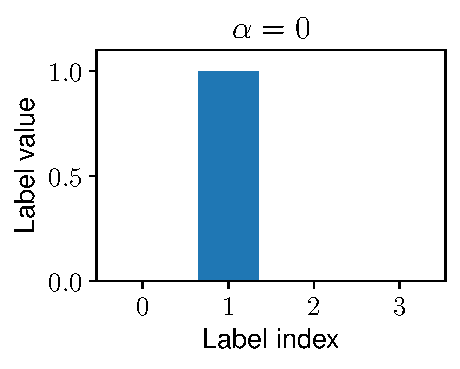
\includegraphics[width=1\linewidth]{figures/ls_plot_0.pdf}
    \end{subfigure}
    \begin{subfigure}{0.32\textwidth}
        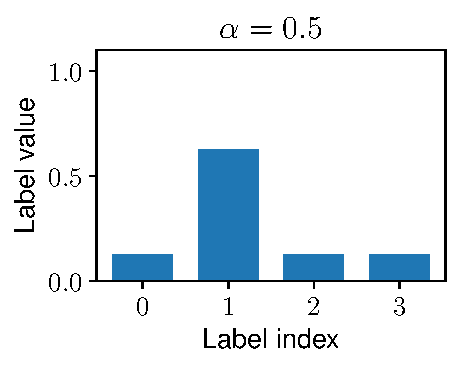
\includegraphics[width=1\linewidth]{figures/ls_plot_1.pdf}
    \end{subfigure}
    \begin{subfigure}{0.32\textwidth}
        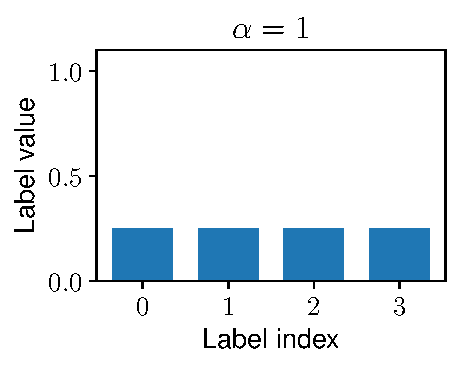
\includegraphics[width=1\linewidth]{figures/ls_plot_2.pdf}
    \end{subfigure}
    \caption{Visualization of different label smoothing constants on a hard label vector with class 1.}
    \label{fig:lab_vis}
\end{figure}
The impact of label smoothing on a hard label vector is demonstrated in Figure \ref{fig:lab_vis}. As $\alpha$ increases, the smooth label vector becomes more uniform. Compared to other methods, label smoothing has a negligible effect on training duration since it only modifies the label vector.

\section{Overview Of Models and Datasets}
A summary of our experiments is presented in Table \ref{tab:overview_short}, which outlines the different combinations of datasets and architectures that were utilized. A more detailed overview is given in the Appendix (see Table \ref{tab:overview}).
\begin{table}[ht]
		\centering
		\caption{Overview of all considered model and dataset combinations.}
		\footnotesize		
        \renewcommand{\arraystretch}{1.4}
        \begin{tabular}{|l|l|}
        \hline\sc Architecture & \sc Datasets \\
        \hline
        \sc \hyperref[fc_model]{FCN } & \sc \hyperref[mnist]{MNIST}, \sc \hyperref[emnist]{EMNIST}, \sc \hyperref[fmnist]{FMNIST} \\
         \sc \hyperref[alexnet_model]{Alexnet} & \sc \hyperref[cifar10]{CIFAR-10} \\
         \sc \hyperref[resnet34_model]{ResNet-34} & \sc \hyperref[cub200]{Cub-200-2011} \\
         \sc \hyperref[resnet50_model]{ResNet-50} & \sc \hyperref[imagenet]{Tiny ImageNet} \\
         \sc \hyperref[resnet56_model]{ResNet-56} & \sc \hyperref[cifar10]{CIFAR-10}, \sc \hyperref[cifar100]{CIFAR-100} \\
          \sc \hyperref[transformer_model]{Transformer} & \sc \hyperref[multi30k]{Multi30k} \\
          \hline
        \end{tabular}
        \label{tab:overview_short}
\end{table}
\subsection{Datasets}
In order to demonstrate the positive impact of label smoothing, the authors made use of five distinct networks and datasets. To validate their findings, we replicated the reported results as closely as possible. To further strengthen the points made by the authors, we also trained additional networks on a multitude of other datasets.

\subsubsection{MNIST} \label{mnist}
The authors used the standard \textit{MNIST} dataset \cite{lecun1998} with $28\times28$ pixel images and ten different label classes. Here, the full $60,000$ training images were used for training, and the $10,000$ test images were used to show the results. For training, the images were randomly shifted by 2 pixels in the x and y directions, and no standardization was used.

\subsubsection{Extended MNIST (EMNIST)}\label{emnist}
The \textit{Extended MNIST} dataset \cite{cohen2017} extends the standard MNIST dataset to also include lowercase and uppercase letters while keeping the structure of $28\times 28$ pixel images. Whereas the original dataset includes all $62$ classes, the subset we used includes only $47$ balanced classes for a total of $112,800$ training and $18,800$ test images. In this balanced dataset, some lowercase letters were removed since they were too similar to their corresponding uppercase letter. In our experiments, we also kept the augmentation from the standard MNIST dataset.

\subsubsection{FMNIST}\label{fmnist}
The \textit{FMNIST} dataset \cite{xiao2017} reimagines the standard MNIST dataset to contain ten classes of fashion products while keeping the structure of $28\times 28$ pixel images. Like the standard MNIST dataset, FMNIST also includes $60,000$ training and $10,000$ test images. In our experiments, we also kept the augmentation from the standard MNIST dataset.

\subsubsection{CIFAR-10} \label{cifar10}
The authors used the standard CIFAR-10 dataset \cite{krizhevsky2009} with $32\times32$ pixel images and ten different label classes. While the original dataset consists of $50,000$ training images and $10,000$ test images, the authors only used $40,000$ images for training and the remaining $10,000$ training images to show results. All images were standardized per image. This means that the color values of each image were subtracted by their mean and divided by their standard deviation. Also, each image from the training dataset was augmented using random horizontal flips and random crops of the original $32\times32$ image to a $24\times24$ image. In our experiments, we kept most augmentation methods but used per-channel instead of per-image standardization. Furthermore, we used the full $50,000$ training images and the $10,000$ test images to show the results.

\subsubsection{CIFAR-100} \label{cifar100}
The authors also used the standard CIFAR-100 dataset \cite{krizhevsky2009} with $32\times32$ pixel images and $100$ different label classes. The same split, standardization, and augmentation as for CIFAR-10 were used. Instead of the random crops from $32\times32$ to $24\times24$ pixels, padded $40\times40$ pixel images were used with random crops to $32\times32$ pixels.

\subsubsection{CUB-200-2011} \label{cub200}
The Caltech-UCSD Birds-200-2011 Dataset \cite{wah2011} or more commonly known as CUB-200-2011 is an extended version of the CUB-200 dataset \cite{welinder2010}. It contains a total of $11,788$ images, of which $5994$ are used for training and $5794$ for testing. There are a total of $200$ classes, each representing a different bird species. Further, there are also annotations for each image, including part locations, binary attributes, and bounding boxes, which are not used in the classification. For the data augmentation, we employed random affine rotations with up to $45$ degrees, random affine translations up to $0.35$, and affine scaling between $0.65$ and $1.35$. As the images do not have a uniform size or aspect ratio in the dataset, we then resized them to $256 \times 256$ pixels. Lastly, there is a $50\%$ chance that the image is flipped horizontally.

\subsubsection{Tiny ImageNet} \label{imagenet}
The authors used the well-known ImageNet/ILSVRC dataset with $224\times224$ images, which each belong to one of $1000$ distinct classes. Due to the considerable size of approximately $1.2$ million images and the training time required, this was out of the feasible range for our available resources. Instead, we made use of Tiny ImageNet, which uses $64 \times 64$ sized samples from ImageNet and $200$ selected classes. The Tiny ImageNet dataset contains $100,000$ training images, $10,000$ validation images, and $10,000$ test images, which aligns better with our rather restricted resources. Tiny ImageNet was introduced as a classification challenge \cite{ali2017}, and the original dataset can be found at the Stanford University website\footnote{\url{http://cs231n.stanford.edu/tiny-imagenet-200.zip}}.
Analog to CUB-200-2011, we made use of affine rotations up to $7.5$ degrees, affine translations up to $0.1$, and affine scaling between $0.925$ and $1.075$. Each image then has a $50\%$ chance to be flipped horizontally.

\subsubsection{Multi30k} \label{multi30k}
The authors used the WMT 2014 English to German dataset \cite{bojar2014}, which consists of around $4.5$ million sentence pairs. Due to training time requirements and memory constraints, we had to fall back to the much smaller Multi30k dataset \cite{elliott2016}. It contains images with descriptions in English and German. We only used the descriptions in training a Transformer model for language translation. 

\subsection{Neural Network Models and Training}
While the authors used TensorFlow \cite{Abadi2016} to implement the networks, we re-implemented these networks in PyTorch \cite{Paszke2019} to ensure both comparability and enhance accessibility. We used the original paper's structure, parameters, settings, and training methods whenever they were given and applicable.

\subsubsection{Fully-connected Network (FCN)}\label{fc_model}
The authors conducted their initial experiment on knowledge distillation using a standard neural network. This network had two hidden layers and utilized ReLU activation, as outlined in \cite{hinton2015}. The network was used in two different variants, with $1200$ and $800$ neurons in each hidden layer, respectively. Although the authors did not provide specific values for dropout, we used $0.5$ based on information found in \cite{hinton2012}.

For training the network, we first used a batch size of $512$ because it massively boosts performance without impacting the accuracy of the network, even though the authors do not state the usage of batches. We trained for $100$ epochs and linearly decreased the learning rates from $1$ in the first layer and $0.1$ in the second layer to $0$. We also used stochastic gradient descent, which was not explicitly stated in the paper, with momentum and dampening of $0.9$. These parameters correspond to the mentioned gradient smoothing. We used cross-entropy loss as a loss function.

\subsubsection{AlexNet}\label{alexnet_model}
The authors' implementation of AlexNet differs significantly from the original version \cite{krizhevsky2012}. In contrast to the five convolutional layers with up to 384 channels used in the original, the authors employ only two convolutional layers with a maximum of 64 channels. Additionally, the linear layers are also altered to accommodate the changes in the convolutional layers.
This deviation is due to the fact that the model is solely intended for use with CIFAR-10 images that are $24\times24$ pixels in size. In contrast, the original AlexNet was created for ImageNet with images of size $224\times224$ pixels.

For training the network on CIFAR-10, we first used a batch size of $128$ and trained for $1246$ epochs or $389,998$ iterations. We used stochastic gradient descent without momentum and implemented a learning rate scheduler starting with a learning rate of $0.1$ and dropping by a factor of $10$ at epochs $415$ and $830$, respectively. Additionally, weight decay of $4\cdot 10^{-2}$ was employed for the last two fully-connected layers, and the used cross-entropy loss was multiplied by a factor of $3$, as suggested by the authors.

\subsubsection{ResNet-34}\label{resnet34_model}
For the classification on the Cub-200-2011 dataset, the official implementation of ResNet-34 in PyTorch\footnote{\url{https://pytorch.org/vision/main/models/resnet.html}\label{note1}} was used with the pre-trained weights for ImageNet. The PyTorch implementation is based on the original ResNet paper \cite{he2016b}.

For the training of Cub-200-2011, we used stochastic gradient descent with a learning rate of $0.3$ and weight decay of $10^{-5}$ for a total of $250$ epochs. Additionally, we applied a scheduler that multiplies the learning rate by $0.9$ every $10$ epochs. Each batch contained $256$ images.

\subsubsection{ResNet-50}\label{resnet50_model}
Analog to ResNet-34, the official implementation of ResNet-50 in PyTorch\footref{note1} was utilized with the pre-trained weights V2 for ImageNet. The PyTorch implementation is based on the original ResNet paper \cite{he2016b}.

For the training of Tiny ImageNet, we utilized stochastic gradient descent with a learning rate of $0.004$ with a weight decay of $10^{-5}$ and a momentum of $0.9$ for a total of $100$ epochs. Furthermore, we applied a scheduler that multiplies the learning rate by $0.5$ every $7$ epochs.

\subsubsection{ResNet-56}\label{resnet56_model}
For the ResNet-56 architecture, the authors use a modified official TensorFlow implementation. This version is based on the ResNet implementation for CIFAR-10 from the original ResNet paper \cite{he2016b} but with preactivation added (as described in \cite{he2016}). For CIFAR-100, the implementation also uses a convolution with filter size $7\times7$, while the standard filter size of $3\times3$ is used for CIFAR-10.

For both training on CIFAR-10 and CIFAR-100, we used the same methods. As stated in the paper, we used batches of $128$ and trained for $205$ epochs or $64,165$ iterations. We used stochastic gradient descent for training, incorporating a Nesterov momentum of $0.9$. Additionally, we implemented a learning rate scheduler starting with a rate of $0.1$ and decreasing by a factor of $10$ at epochs $102$ and $153$. We also used weight decay of $10^{-4}$ and multiplied the used cross-entropy term by a factor of $3$, as recommended in the paper. Finally, we utilized gradient clipping with a maximum threshold of $1$.

\subsubsection{Transformer}\label{transformer_model}
The Transformer is an encoder-decoder network architecture introduced in 2017 by Vaswani et al. \cite{vaswani2017}. It is based upon the so-called attention mechanism. The attention mechanism is responsible for capturing relationships between words in a sequence. It allows the model to assign values to each word pair while processing the input. This value represents the relationship between the two words. Thanks to this, transformers can efficiently process long-range dependencies and achieve state-of-the-art performance in various natural language processing tasks.
The authors use the original Transformer architecture \cite{vaswani2017} with the same hyperparameters for exploring the effects of label smoothing on a language translation task. We use the sequence-to-sequence model implemented by PyTorch in their example for language translation using transformer \cite{transformerTutorial}. It is a down-scaled version of the original transformer network. This model has three encoder and decoder layers instead of six, while also using 512 instead of 2048 dimensions for the inner feed-forward networks.

\section{Accuracy with Label Smoothing}\label{sec:acc}
In the original work, the authors claimed that label smoothing has a positive impact on the test accuracy of a trained network. For this, multiple examples were provided, where networks were trained with varying values of the label smoothing constant $\alpha$.

\begin{table}[ht]
    \centering
    \caption{Top-1 classification accuracies of networks trained with and without label smoothing compared with the results from Müller et al. \cite{mueller2019}. Best results are printed \textbf{bold}.}
    \footnotesize
    \renewcommand{\arraystretch}{1.4}
    \begin{tabular}{|l|l|ccccc|}
            \hline
            & &\multicolumn{5}{c|}{\sc Accuracy [\%]} \\
            \sc Dataset & \sc Architecture & $\mathrm{\alpha = 0.0}$ & $\mathrm{\alpha = 0.05}$ & $\mathrm{\alpha= 0.1}$ & $\mathrm{\alpha=0.15}$ &$\mathrm{\alpha = 0.30}$\\
            \hline
            MNIST & \sc{FCN (ours)} & 99.06 & $99.33$ & 99.31 & 99.24 & 99.13\\
            EMNIST & \sc {FCN (ours)} & 88.79 & 89.11 &$89.35$& 89.19 & 88.88\\
            FMNIST & \sc{FCN (ours)} & $91.01$ & 90.66 & 90.45 & 90.59 & 90.37\\
            \hline
            & \sc AlexNet \cite{mueller2019}& $86.8$ & - & 86.7 & - & -\\
            CIFAR-10 & \sc AlexNet (ours)& 85.01 & 85.13 & 85.47 & 84.83 &  $86.02$\\
            & \sc ResNet-56 (ours)& 93.59 & ${93.62}$ & 93.33 & 93.55 & 93.53\\
            \hline
            \multirow{2}{*}{CIFAR-100} & \sc ResNet-56 \cite{mueller2019} & 72.1 & - & $72.7$ & - & -\\
            & \sc ResNet-56 (ours)& 71.61 & 71.99 & $72.07$ & 71.74 & 71.75\\
            \hline
            \sc CUB-200-2011 & \sc ResNet-34 (ours) & 77.75 & 80.38 & 80.48 & $81.12$ & 80.77\\
            \hline
            \sc TinyImageNet & \sc ResNet-50 (ours) & 72.20 & 72.65 & 72.30 & 72.28 & $72.75$\\
            \hline
            \sc ImageNet & \sc Inception-v4 \cite{mueller2019} & $80.9$ & - & $80.9$ & - & -\\
            \hline
    \end{tabular}
    \label{tab:acc}
\end{table}

As shown in Table \ref{tab:acc} we were able to verify these results and observed the same trend for additional architectures and datasets.
Our extensive evaluation shows that implementing moderate levels of label smoothing can effectively reduce overfitting and increase the accuracy of the networks overall. The level of label smoothing required to effectively mitigate overfitting and improve accuracy varies between architectures and datasets. While some models benefit significantly from high label smoothing constants (e.g., AlexNet on CIFAR-10), others only exhibit minor improvements or even degradation from small constants (e.g., ResNet-56 on CIFAR-10 / FCN on FMNIST).

\section{Penultimate Layer Representation}\label{sec:plr}
The authors propose a visualization scheme that illustrates how label smoothing affects the activations of the penultimate layer and the output of the network.
For a single data point, neural network classifiers calculate a prediction \begin{equation}
    p_k = \frac{\exp{(a^T w_k)}}{\sum_{l=1}^K \exp{(a^T w_l)}}\label{eq:softmax}
\end{equation} for the $k$-th class by applying the softmax to the logit $a^Tw_k$, where $a\in \mathbb{R}^{n}$ is the activation vector of the penultimate layer and $w_k$ is the weight vector for the $k$-th class of the last layer. The weight vector $w_k\in \mathbb{R}^{n}$ can be seen as a template of class $k$.
The authors state, that the logits depend on the Euclidean distance $||a-w_k||^2$ between the activations of the penultimate layer $a$ and the template $w_k$. 
To visualize a high-dimensional activation $a$ in two dimensions, we first choose three classes and their corresponding templates $w_1, w_2$, and $w_3$. To find the plane passing through the templates, we subtract the third template from the first and second template, resulting in vectors $\Delta_1 = w_1 - w_3$ and $\Delta_2 = w_2 - w_3$. 
After that, we define the matrix 
\begin{align*}
A &= \begin{bmatrix}
           \Delta_1~\Delta_2 \\
     \end{bmatrix}\in \mathbb{R}^{n\times 2},
\end{align*}
which contains the vectors  $\Delta_1$ and $\Delta_2$ as columns. Next, we  orthogonalize $A$ by calculating its QR decomposition $A= QR$, where $Q\in\mathbb{R}^{n\times 2}$ is an orthogonal matrix  and  $R \in \mathbb{R}^{2 \times 2}$ is an upper triangular matrix. After normalizing the column vectors of $Q$, we obtain two vectors $u \in \mathbb{R}^n$ and $v \in \mathbb{R}^n$, which are orthogonal vectors that form the basis of a two-dimensional vector subspace. We can project the activation now into the subspace. The subspace coordinates are given by $\lambda=a^Tu$ and $\mu=a^Tv$.

For the visualization, we choose a number of data points from the three picked classes and produce a scatter plot of their subspace coordinates. A possible implementation can be found in Section \ref{sec:app_pen}.
According to Müller et al.~\cite{mueller2019}, label smoothing promotes the tendency for the activations of the second-to-last layer to align closely with the reference pattern of the accurate class, while maintaining an equitable separation from the reference patterns of the inaccurate classes.

\definecolor{pl_red}{RGB}{255, 12, 12}
\definecolor{pl_green}{RGB}{0, 128, 0}
\definecolor{pl_blue}{RGB}{0, 0, 255}

\subsubsection{Results}
We were able to reproduce the effect described in the paper as seen in Figure \ref{fig:pen}. For CIFAR-10, we chose the classes airplane ({\color{pl_red}red}), automobile ({\color{pl_green}green}), and bird ({\color{pl_blue}blue}). For CIFAR-100, we chose apple ({\color{pl_red}red}), aquarium\_fish ({\color{pl_green}green}), and baby ({\color{pl_blue}blue}). For MNIST, we chose zero ({\color{pl_red}red}), one ({\color{pl_green}green}), and two ({\color{pl_blue}blue}). The effect on the clusters is clearly visible, as when training with label smoothing, the clusters become much denser and equidistant (i.e., the shape is more triangular). Also, the distance between the templates is much smaller, which can be seen by looking at the scale of the axes.

\newcolumntype{C}{>{\centering\arraybackslash\small}m{.24\linewidth}}
\begin{figure}[ht]
\centering
        {\setlength{\tabcolsep}{0em}\begin{tabular}{m{.03\linewidth}*4{C}@{}}
        
             & Training w/o LS & Training w/ LS & Validation w/o LS & Validation w/ LS \\ 
            \rotatebox[y=3em]{90}{\small CIFAR-10} 
            & 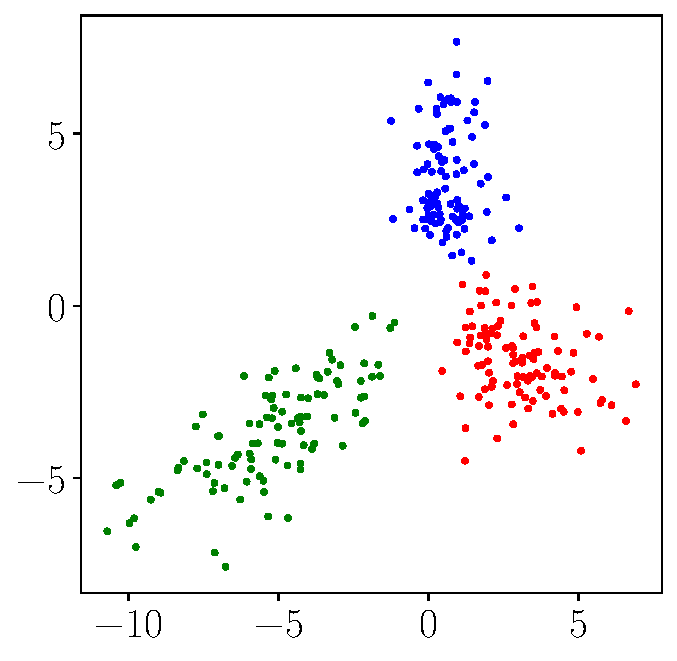
\includegraphics[width=\linewidth]{figures/alexnet_penultimate_plot_1.pdf} 
            & 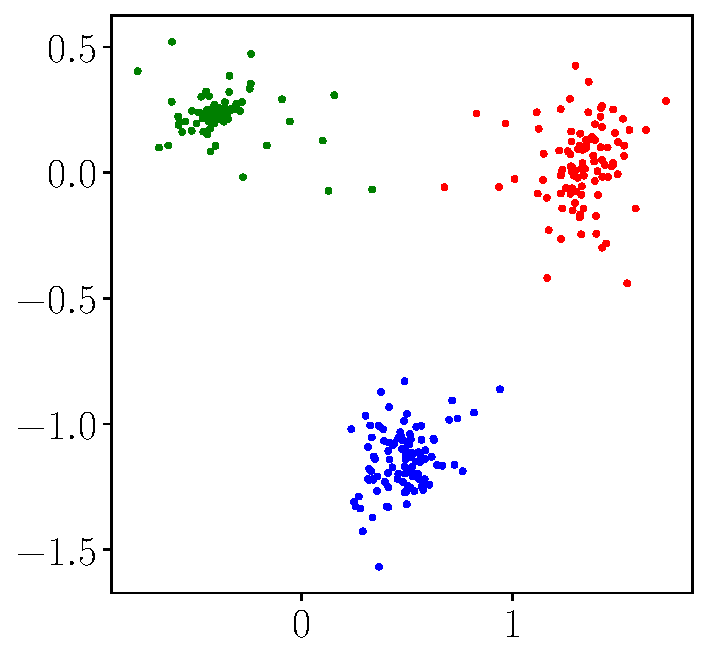
\includegraphics[width=\linewidth]{figures/alexnet_penultimate_plot_3.pdf} 
            & 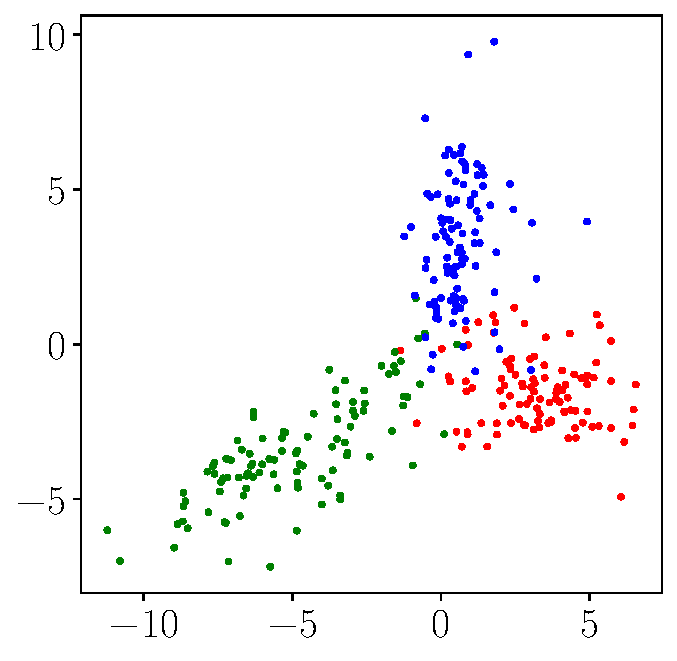
\includegraphics[width=\linewidth]{figures/alexnet_penultimate_plot_0.pdf} 
            & 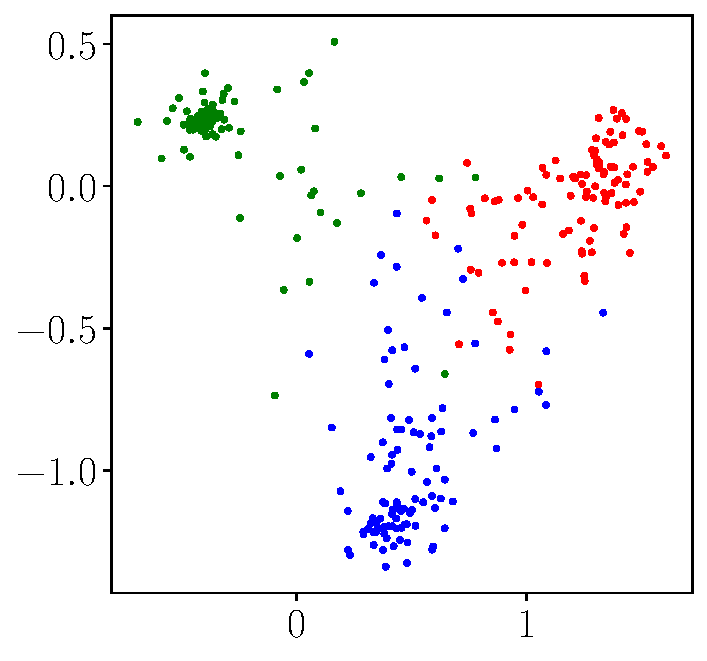
\includegraphics[width=\linewidth]{figures/alexnet_penultimate_plot_2.pdf}\\ 
            \rotatebox[y=3em]{90}{\small CIFAR-100} 
            & 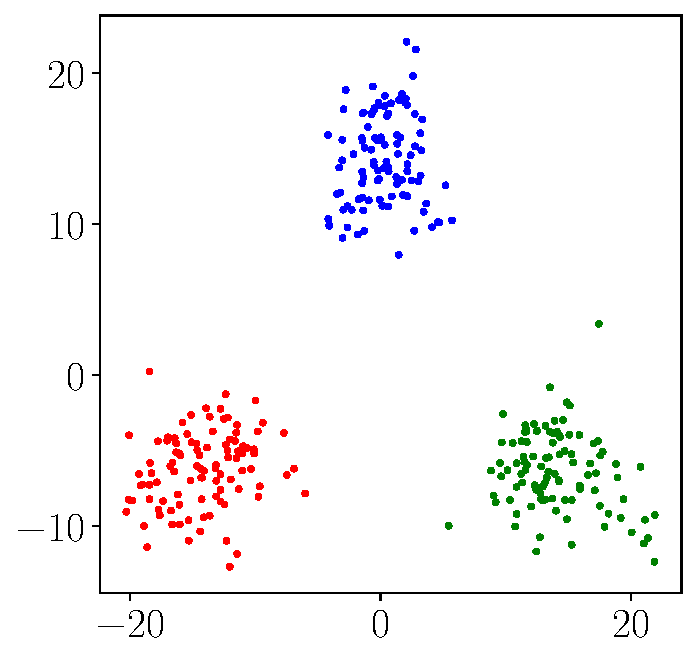
\includegraphics[width=\linewidth]{figures/resnet_penultimate_plot_1.pdf} 
            & 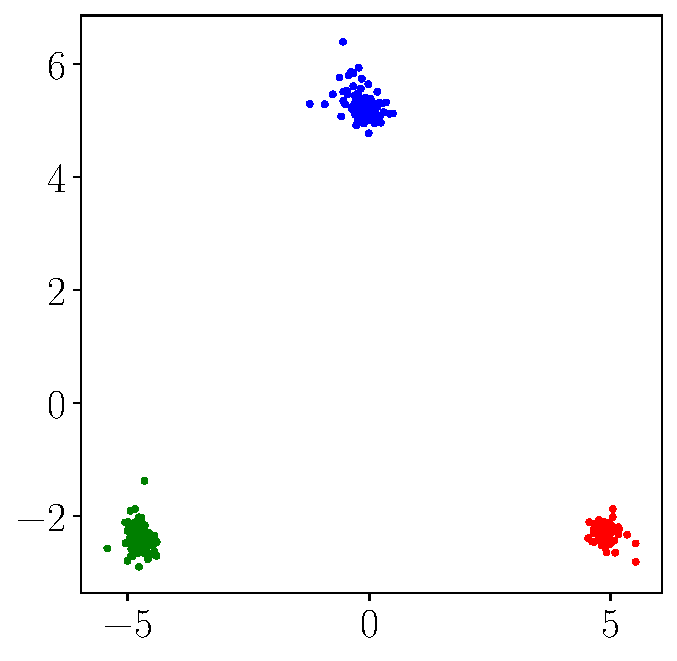
\includegraphics[width=\linewidth]{figures/resnet_penultimate_plot_3.pdf} 
            & 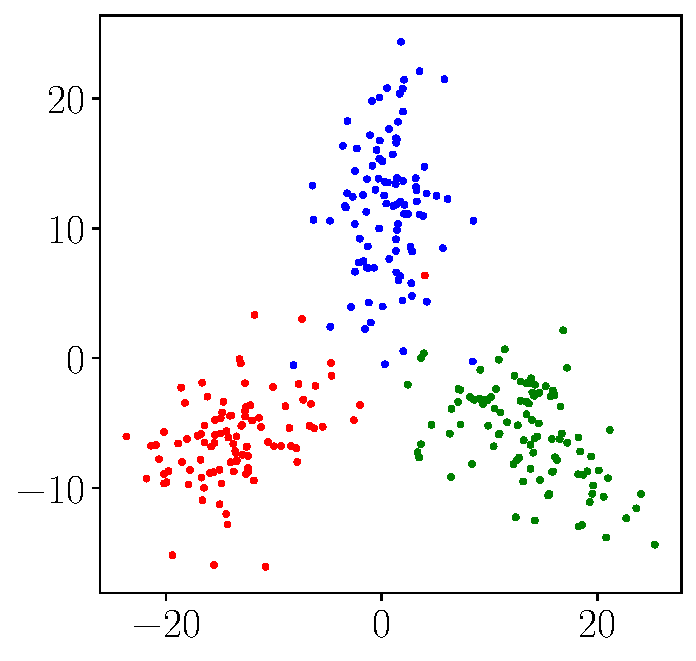
\includegraphics[width=\linewidth]{figures/resnet_penultimate_plot_0.pdf} 
            & 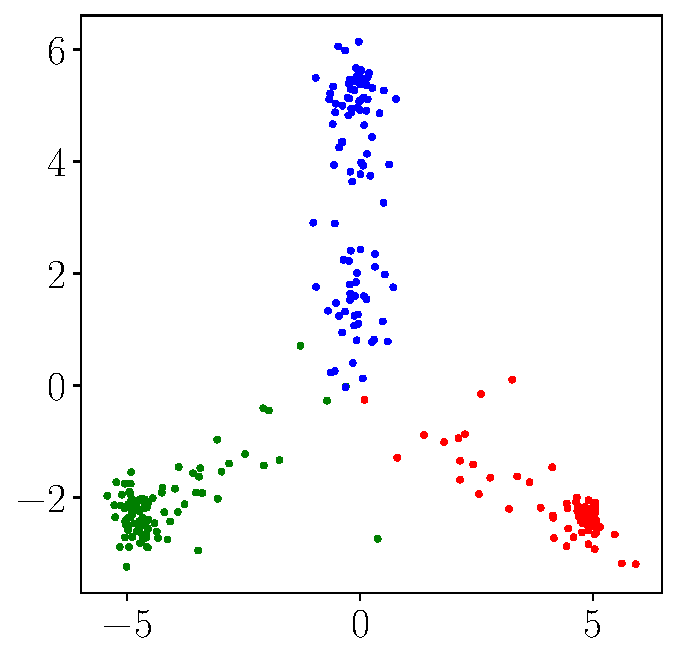
\includegraphics[width=\linewidth]{figures/resnet_penultimate_plot_2.pdf}\\ 
            \rotatebox[y=3em]{90}{\small MNIST} 
            & 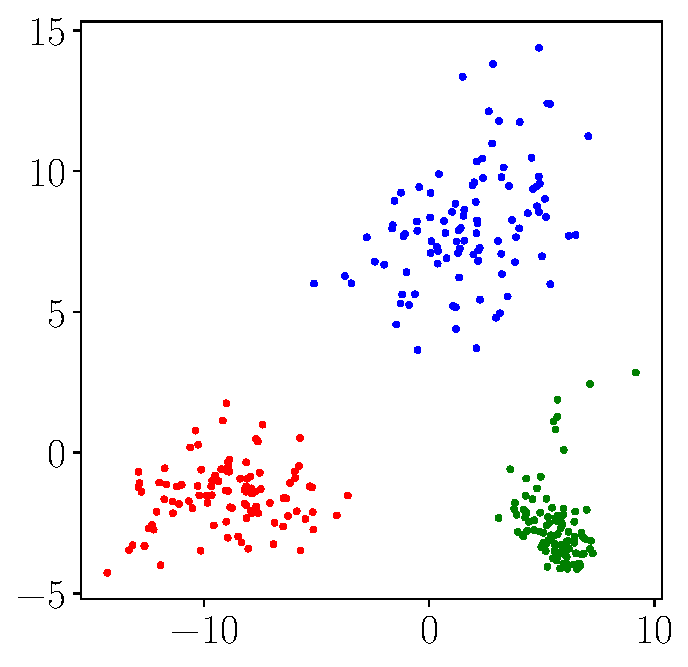
\includegraphics[width=\linewidth]{figures/fc_penultimate_plot_1.pdf} 
            & 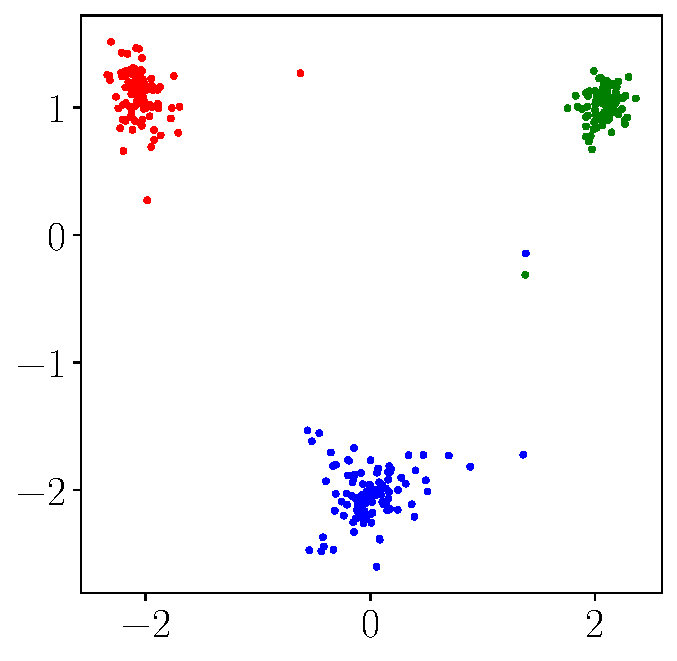
\includegraphics[width=\linewidth]{figures/fc_penultimate_plot_3.pdf} 
            & 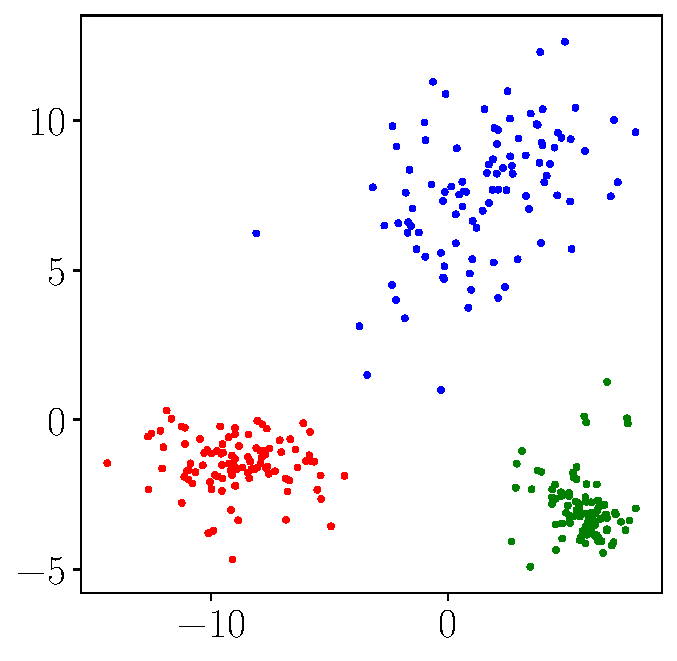
\includegraphics[width=\linewidth]{figures/fc_penultimate_plot_0.pdf} 
            & 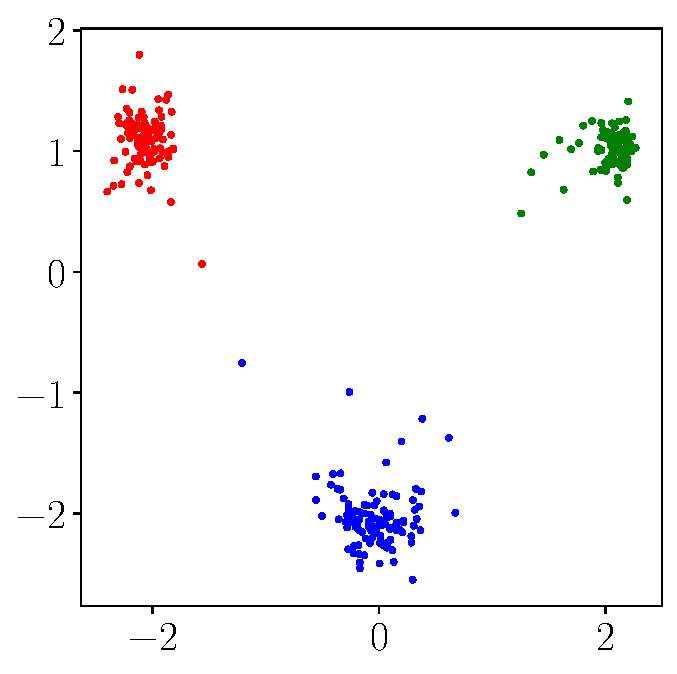
\includegraphics[width=\linewidth]{figures/fc_penultimate_plot_2.pdf}\\ 
        \end{tabular}}
        
        \caption{Visualization of the penultimate layer activations: AlexNet on CIFAR-10 (first row), ResNet-56 on CIFAR-100 (second row), FCN on MNIST (third row).}
        \label{fig:pen}
\end{figure}


\section{Implicit Model Calibration}\label{sec:imc}
\label{sec:model_calibration_basics}
The authors compared the model calibration of multiple models trained with hard labels and smooth labels to demonstrate the improvement of results with smooth labels. Additionally, they applied temperature scaling to the models trained with hard labels to improve their calibration. The evaluation was performed using the \textit{expected calibration error (ECE)}, followed by the corresponding reliability diagrams.\\

In the original paper, the model calibration was examined on ResNet-56, InceptionV4, and the Transformer architecture. While ResNet-56 and InceptionV4 were used for classification on the CIFAR-100 and ImageNet datasets, the Transformer was trained on the Multi30k dataset to translate text from English to German.

One of the primary objectives of label smoothing is to improve the calibration of neural networks. The calibration can be described as the difference between accuracy and confidence. A poorly calibrated network exhibits a high difference, while a well-calibrated network shows a low difference. While the accuracy of a network is a common measure, confidence is primarily evaluated in the context of model calibration. The confidence for a given input example $x$ is given by the highest output provided by the network on that input through
$$\conf(x) = \max_k\{p_k(x)\},$$
where $p_k$ is the $k$-th output of the neural network.

A technique that is frequently used to calibrate a trained network is \textit{temperature scaling} \cite{Guo2017}. Temperature scaling applies a temperature $\tau>0$ to the logits before applying the softmax normalization as described by
$$p_k^{\tau} = \frac{\exp(z_k/\tau)}{\sum_{i=1}^K \exp(z_i/\tau)},$$
where $p_k$ refers to the $k$-th prediction and $z_k$ refers to the $k$-th logit of the network. Thus each logit is divided by the temperature before the softmax normalization is applied. This technique is used to explicitly calibrate a network, as it only affects the confidence without impacting the accuracy. Using a high temperature $(\tau > 1)$ decreases the confidence while employing a low temperature $(\tau < 1)$ would increase the confidence. When $\tau=1$ is used, temperature scaling has no effect, as it effectively becomes a division by $1$.\\

A common index to measure the calibration of a network is the \textit{expected calibration error (ECE)} \cite{Naeini2015}. This index estimates the calibration of a network based on a set of test examples. To calculate the ECE, the output of the network is calculated over every example, and these are then separated into $B$ distinct bins according to their confidence. For example, the bin $b$ would include all examples $x$, where $\conf(x) \in \left\lbrack\frac{b}{B}, \frac{b+1}{B}\right)$. Over each of those bins, the ECE can be calculated like
$$ECE = \sum_{b=1}^B \frac{n_b}{N} |\conf(b)-\acc(b)|,$$
where $n_b$ is the number of examples in bin $b$, $N$ is the total amount of samples, $\conf(b)$ is the average confidence over all examples in $b$ and $\acc(b)$ is the accuracy over all examples in $b$. In general, a lower ECE is preferred and indicates a better calibrated network.\\

One way to visualize the calibration is a confidence-accuracy plot or \textit{reliability diagram}. For the diagram, the bins are calculated as above, along with their confidence and accuracy. Each bin then correlates to a point in a confidence-accuracy plot, providing a more detailed description of the network calibration. In the optimal case, each of the bin's accuracy and confidence values would be equal, resulting in a straight line. In such a case, the network would be perfectly calibrated, as the confidence and accuracy always align. For the following plots and ECE computations, the number of bins is consistently set to $15$ to align with the original paper.

\subsection{Model Calibration for Classification}

In this experiment, we compared the ECE for several network architectures on different datasets. To further examine the impact of different degrees of label smoothing on the calibration, we used several different label smoothing constants for each network. Following the methodology of the original paper, the models trained on hard labels were also improved by temperature scaling and compared with the other models. While the experiment in the original paper only evaluated three different architectures, we took a more quantitative approach and evaluated several additional combinations of different architectures and datasets. This evaluation thus allows a much broader understanding of the effects of label smoothing on network calibration.


\begin{table}
    \centering
    \caption{ECE for neural networks trained with and without label smoothing compared with temperature-scaled networks and the results from Müller et al. \cite{mueller2019}. Best results are printed \textbf{bold}.}
    \footnotesize
    \renewcommand{\arraystretch}{1.4}
    \setlength{\tabcolsep}{3pt}
    \begin{tabular}{|l|l|cc|ccccc|}
        \hline
        & & \multicolumn{2}{c|}{} & \multicolumn{5}{c|}{\sc ECE} \\
        \cline{3-9}
        & & \multicolumn{2}{c|}{$\mathrm{\alpha=0.0}$} & $\mathrm{\alpha=0.0}$ & $\mathrm{\alpha=0.05}$ & $\mathrm{\alpha=0.1}$ &$\mathrm{\alpha=0.15}$ & $\mathrm{\alpha=0.3}$\\  
        \cline{3-9}
        \sc Dataset & \sc Architecture & ECE & T & $\mathrm{T=1.0}$ & $\mathrm{T=1.0}$ & $\mathrm{T=1.0}$ & $\mathrm{T=1.0}$ & $\mathrm{T=1.0}$\\
        \hline
        MNIST & \sc FCN (ours) & 0.001 & 1.06 & $0.002$ & 0.056 & 0.102 & 0.147 & 0.281\\
        EMNIST & \sc FCN (ours) & 0.008 & 1.14 & $0.017$ & 0.056 & 0.108 & 0.154 & 0.288\\
        FMNIST & \sc FCN (ours) & 0.008 & 1.1 & $0.010$ & 0.042 & 0.085 & 0.128 & 0.252\\
        \hline
        \multirow{2}{*}{CIFAR-10} & \sc AlexNet (ours)& 0.012 & 2.5 & 0.097 & $0.026$ & 0.048 & 0.087 & 0.221\\
        & \sc ResNet-56 (ours) & 0.006 & 3.1& 0.049 & $0.028$ & 0.065 & 0.102 & 0.222\\
        \hline
        \multirow{2}{*}{CIFAR-100} & \sc ResNet-56 (ours)& 0.029 & 2.9 & 0.207 & 0.053 & $0.043$ & 0.045 & 0.120\\
        & \sc ResNet-56 \cite{mueller2019}& 0.021 & 1.9 & 0.150 & $0.024$ & - & - & -\\
        \hline
        CUB-200-2011 & \sc ResNet-34 (ours)& 0.013 & 1.4 & $0.082$ & 0.159 & 0.235 & 0.286 & 0.400\\
        \hline
        TinyImageNet & \sc ResNet-50 (ours)& 0.013 & 1.7 & 0.150 & 0.060 & $0.045$ & 0.054 & 0.166\\
        \hline
        ImageNet & \sc InceptionV4 \cite{mueller2019}& 0.022 & 1.4 & 0.071 & - & $0.035$ & - & -\\
        \hline
        Multi30k & \sc Transformer (ours) & 0.058 & 1.8 & 0.449 & 0.475 & 0.372 & 0.222 & $0.110$ \\
        \hline
    \end{tabular}
    \label{tab:ece}
\end{table}

The results of this evaluation are presented in Table \ref{tab:ece}. Here one can see that using small label smoothing constants in training can help to implicitly calibrate a neural network. In most experiments, the ECE became smaller when using label smoothing. Although temperature scaling still remains the best technique when looking at the results, finding a fitting temperature for a network can often be tedious, as it includes evaluating the ECE for every reasonable temperature. But label smoothing does not seem to help in every case. For the fully-connected networks, even small label smoothing constants did not help. This is the case because these networks were not overconfident in their predictions but rather well-calibrated. For these scenarios, label smoothing is not the best method as it makes the network underconfident. This phenomenon can be observed in Figure \ref{fig:acc_conf_resnet56} and \ref{fig:acc_conf_mnist}. 

\begin{figure}[ht]
    \begin{subfigure}{.49\textwidth}
    \centering
    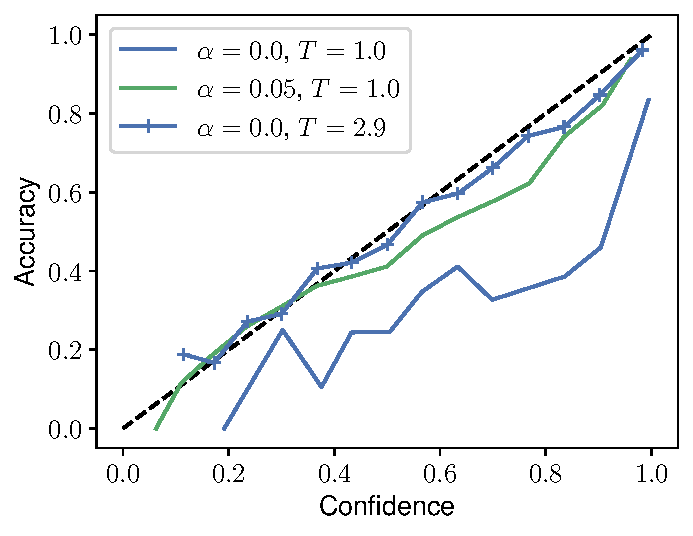
\includegraphics[width=\linewidth]{figures/reliability_resnet.pdf}
    \caption{ResNet-56 on the CIFAR-100 dataset}
    \label{fig:acc_conf_resnet56}
\end{subfigure}
\hfill
\begin{subfigure}{.49\textwidth}
    \centering
    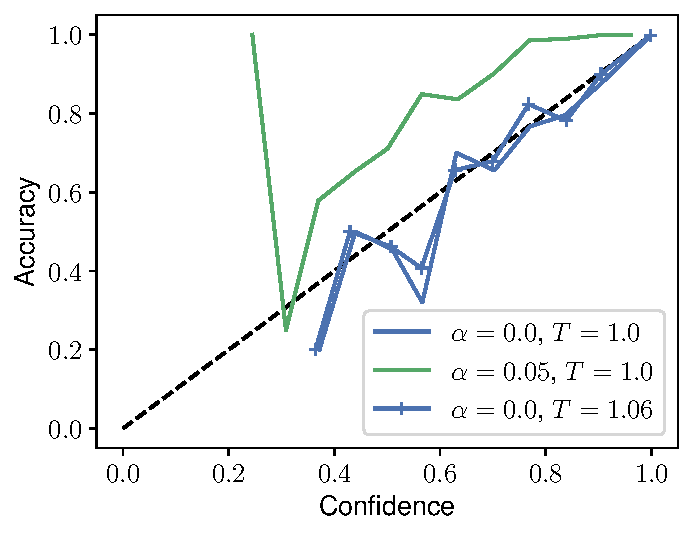
\includegraphics[width=\linewidth]{figures/reliability_mnist.pdf}
    \caption{Fully-connected network on the MNIST dataset}
    \label{fig:acc_conf_mnist}
\end{subfigure}
\caption{Reliability diagrams for classification networks. For ResNet-56, label smoothing resulted in a good calibration, while it caused underconfidence for the fully-connected network.}
\end{figure}

While the ResNet-56 trained with hard labels is rather overconfident (all points lie under the black line), both lines for the network trained with label smoothing and for the temperature-scaled network are very close to the black line and, as such, well-calibrated. For the fully-connected network, both the network trained with hard labels and the temperature-scaled network are rather well-calibrated, but the line for the network trained with label smoothing lies over the black line and, as such, is relatively underconfident.

\subsection{Model Calibration on Transformer}
\begin{wrapfigure}{r}{0.46\textwidth}\vspace{-1.1cm}
    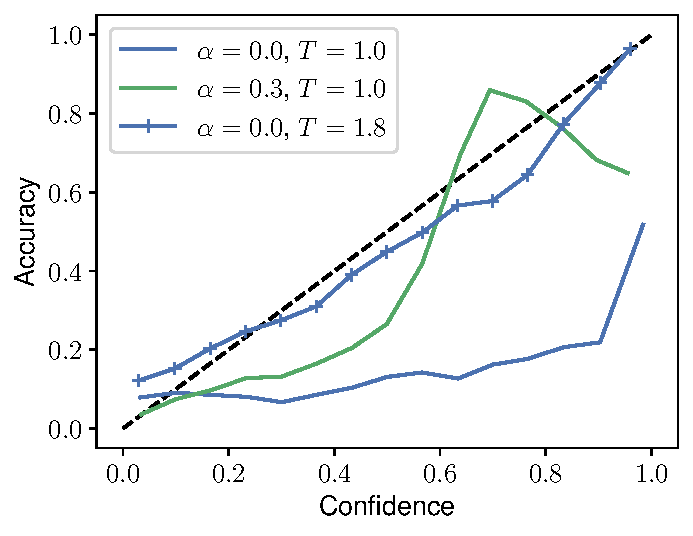
\includegraphics[width=1\linewidth]{figures/transformer_reliability_0.3.pdf}
    \caption{Reliability diagram for Transformer on the Multi30k dataset. Label smoothing caused a significantly better calibration.}
    \vspace{-1cm}
    \label{fig:acc_conf_transformer}
\end{wrapfigure}
When using a Transformer, we were also able to reproduce the trend of achieving a better calibration with label smoothing. When conducting the above experiment on the Transformer, we achieve a substantially better ECE score when label smoothing of $\alpha = 0.3$ is applied, which can be seen in Table \ref{tab:ece}. The same trend can be found in the corresponding reliability diagram (see Figure \ref{fig:acc_conf_transformer}). But despite the improvements label smoothing provides, it is visible that the positive impact of temperature scaling is still stronger.

\subsection{Translation Quality on Transformer}
The quality of language translations is commonly evaluated using the \textit{bilingual evaluation understudy (BLEU) score} \cite{papineni2002}, which is based on the concept of $n$-grams. $n$-grams are sequences of $n$ consecutive words in a sentence. To compare a generated sentence (also called "candidate") with a reference sentence, the percentage of $n$-grams from the candidate appearing in the reference is calculated. The result is known as the $n$-gram precision. This $n$-gram precision is calculated for all $n$-grams starting with $n = 1$ and ending with a specified maximum, which is typically $n = 4$. The BLEU score is then calculated as a weighted average of the different $n$-gram precision, while also incorporating a brevity penalty. This penalty helps to avoid overly short translations.\\

The \textit{negative log-likelihood (NLL)} is commonly used as a loss function in multi-class classification. It has to be applied after the \textit{softmax} activation function and is defined as
$$l(p, y) = -\log(p_n),$$
where $p_n$ denotes the prediction of the network for the correct class.
The NLL is up to a constant factor equivalent to the cross-entropy loss if no label smoothing is used. If label smoothing is used, it is not equivalent because NLL does not consider the predictions and labels for the incorrect classes.\\

The influence of temperature scaling and label smoothing on the ECE and the BLEU score are shown in Figure \ref{fig:cal_effect_transformer}. Here it can be seen that the amount of temperature scaling needed to get a minimal ECE is decreased to about $1.1$ when a label smoothing constant of $\alpha = 0.3$ is used. This corresponds to the results in the paper. We were not able to reproduce an increase in BLEU score by using label smoothing. In the rightmost panel, the effect on the NLL is plotted. The difference between smooth labels (orange) and hard labels (blue) is not large, but the smooth labels perform slightly better for low temperature values, while this trend reversed for higher ones. This differs from the results from the paper, where the hard labels had a better NLL for all temperatures.

\begin{figure}[ht]
    \centering
    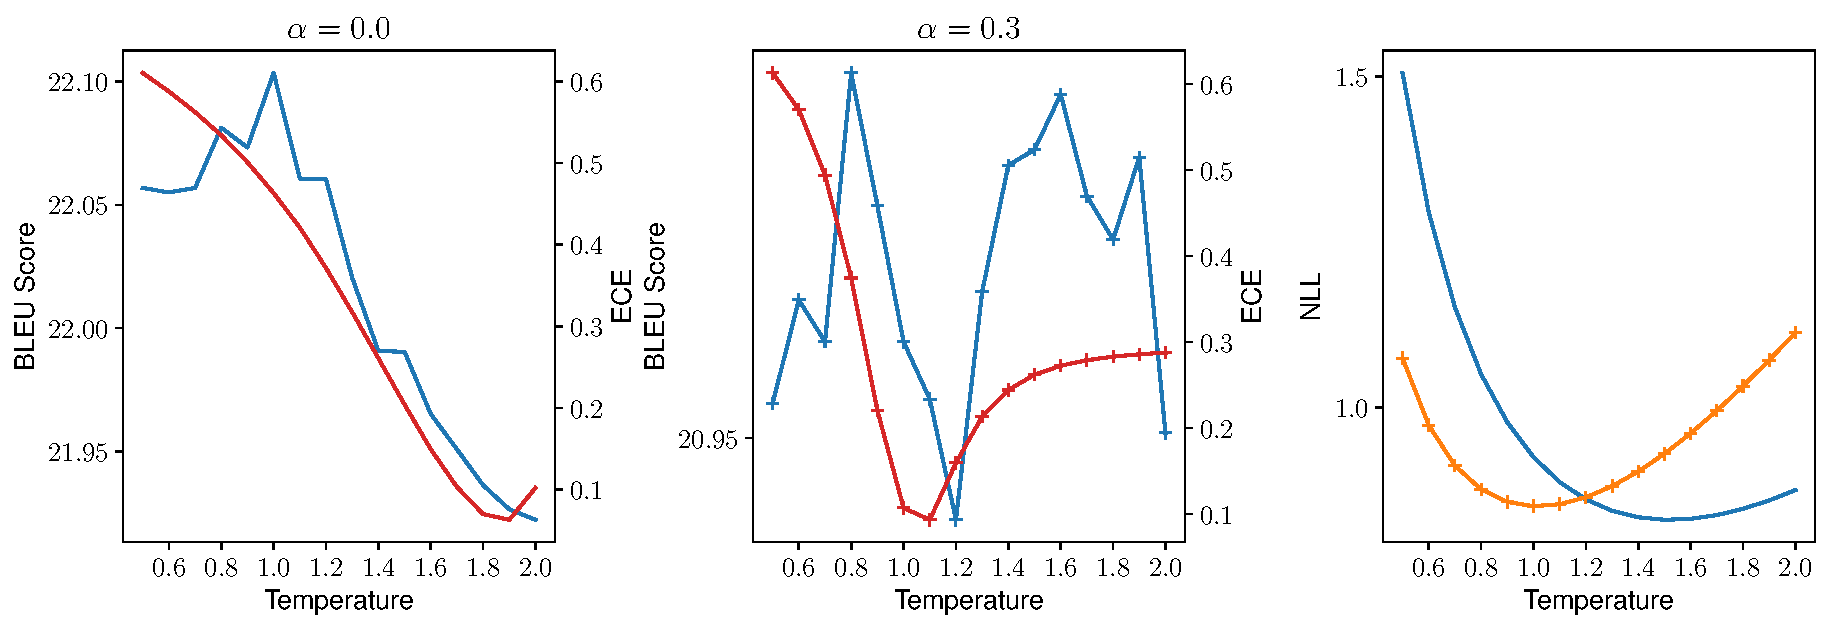
\includegraphics[width=1\linewidth]{figures/transformer_calibrationEffects_0.3.pdf}
    \caption{The effects of calibration on ECE, BLEU, and NLL for Transformer on the Multi30k dataset. In the first two panels, the blue line reflects the BLEU score, and the red line represents the ECE. Curves with markers correspond to networks trained with label smoothing.}
    \label{fig:cal_effect_transformer}
\end{figure}

\section{Knowledge Distillation}\label{sec:kd}
The concept of knowledge distillation \citep{hinton2015} is a common technique to train a small neural network (student) from the outputs of a large neural network (teacher). In this way, it is possible to achieve a higher accuracy of the student network compared to usual supervised training. The rationale is that the knowledge that was extracted by the teacher network can help the training of the student network.  
A usual knowledge distillation procedure works as follows: first, a teacher network is trained as usual. After that, the student network is trained by minimizing the convex combination of two losses
\begin{equation}
    \label{eq:dist_loss}
    L(y, p^\tau, q^\tau)=(1-\beta) H(y,q^\tau) + \beta H(p^\tau, q^\tau),
\end{equation}
where $H$ denotes the cross-entropy, $\beta\in [0,1]$ is a hyperparameter that balances the two losses, and $p^\tau$ and $q^\tau$ are the scaled output probabilities of the teacher network and the student network after temperature scaling with temperature $\tau$ has been applied (refer to Section \ref{sec:model_calibration_basics}). The first term $H(y,q^\tau)$ is the usual cross-entropy between the ground-truth label and the output probabilities of the student network. The second term $H(p^\tau, q^\tau)$ is the cross-entropy between the output probabilities of the student network and the output probabilities of the teacher network.
\begin{figure}[ht]
    \centering
    %\begin{tikzpicture}
%        \node[draw, thick, rounded corners, rectangle] at (2,2.5) (1) {\begin{tabular}{c}
%             \textbf{Original Labels} \\ \textbf{(Hard or Smooth)}
%        \end{tabular}};
%        \node[draw, thick, rounded corners, rectangle split, rectangle split parts=3] at (0.5,0) (2) {Input\nodepart{two}\textbf{Teacher Network}\nodepart{three}Output};
%        \node[draw, thick, rounded corners, rectangle] at (0.5, -2) (4) {\textbf{Temperature Scaling}};
%        \node[draw, thick, rounded corners, rectangle split, rectangle split parts=3] at (2,-4) (3) {Input\nodepart{two}\textbf{Student Network}\nodepart{three}Output};
%        \draw[-Triangle Cap,line width=0.8ex] ([xshift=-9mm] 1.south) to ([xshift=6mm] 2.north);
%        \draw[-Triangle Cap,line width=0.8ex] ([xshift=6mm] 2.south) to ([xshift=6mm] 4.north);
%        \draw[-Triangle Cap,line width=0.8ex] ([xshift=6mm] 4.south) to ([xshift=-9mm] 3.north);
%        \draw[-Triangle Cap,line width=0.8ex] ([xshift=9mm]1.south) to ([xshift=9mm]3.north);
%    \end{tikzpicture}
    \begin{tikzpicture}[scale=0.7, every node/.style={scale=0.7}]
        \node[draw,  rounded corners, rectangle, fill=cyan!20] at (0,0) (data) {            Training inputs};
        \node[draw,  rounded corners, rectangle, fill=cyan!20] at (0,-2.5) (labels) {             Training labels};
        \node[draw,  rounded corners, rectangle, align=center] at (4.5,-1) (teacher) {Teacher network\\(fixed parameters)};
        \node at (9,-1) (teacher-output) {$p^\tau$};
        \node at (9,1) (student-output) {$q^\tau$};
        \node at (11,-1) (loss) {$L$};
        \node at (9,-2.5) (smooth-labels) {$y^\text{LS}$};
        \node[draw,  rounded corners, rectangle, align=center] at (4.5,1) (student) {Student network\\(learnable parameters)};
        \draw[-Latex,line width=0.2ex] (data.east) to (teacher.west);
        \draw[-Latex,line width=0.2ex] (teacher.east) -- node[above,align=center] {\footnotesize Temperature \\[-2pt] \footnotesize scaling} (teacher-output.west);
        \draw[-Latex,line width=0.2ex] (student.east) -- node[above,align=center] {\footnotesize Temperature \\[-2pt] \footnotesize scaling} (student-output.west);
        \draw[-Latex,line width=0.2ex] (labels.east) -- node[above,align=center] {\footnotesize Label smoothing} (smooth-labels.west);
        \draw[-Latex,line width=0.2ex] (data.east) to (student.west);
        \draw[-Latex,line width=0.2ex] (smooth-labels.east) to ([yshift=-2mm]loss.west);        
        \draw[-Latex,line width=0.2ex] (teacher-output.east) to (loss.west);
        \draw[-Latex,line width=0.2ex] (student-output.east) to ([yshift=2mm]loss.west);
%        \draw[-Latex,line width=0.2ex, gray, dashed] (loss.north) to[in=60,out=90, looseness=1.2] (student.north);
    \end{tikzpicture}
    \caption{Knowledge distillation with label smoothing and temperature scaling.}
    \label{fig:distillation_diagram}
\end{figure}
Figure \ref{fig:distillation_diagram} shows the abstract concept of knowledge distillation. Note that the temperature scaling is optional and can be omitted. In the following experiments, the temperature scaling for the student network was not included during its training process, as it is only a scalar that can be learned.

The authors also define a smoothness index 
 \begin{equation}
    \label{eq:dist_smooth}
    \gamma = \mathbb{E}\left\lbrack \sum_{k=1}^K(1-y_k)p_k^\tau K/(K-1)\right\rbrack,
\end{equation}
where $y_k$ is the $k$-th entry of the label-vector, $p_k^\tau$ is the $k$-th component of the teacher output, and $K$ is the number of output classes. This smoothness index allows us to compare models that use different combinations of label smoothing and temperature scaling and is computed over all training examples.

\subsection{Distillation with Fully-connected Networks}

\begin{wraptable}{r}{0.5\textwidth}\vspace{-0.4cm}
\footnotesize
    \centering
    \caption{Errors of the FCN networks trained on MNIST compared to the errors from Müller et al. \cite{mueller2019}.}
    \begin{tabular}{|l|c|c|}
    \hline
        \sc Network & \sc Müller et al. & \sc Ours\\
        \hline
        \sc Teacher w/o LS & 0.67\% & 0.81\%\\
        %\hline
        \sc Teacher w/ LS & 0.59\% & 0.69\%\\
        \hline
        \sc Student w/o LS & 0.74\% & 0.93\%\\
        %\hline
        \sc Student w/ LS & 0.91\% & 1.05\%\\
        \hline
    \end{tabular}
    \label{tab:acc_toy_kd}
\end{wraptable}

In the first experiment, we trained a fully-connected teacher network with $1200$ neurons per layer using dropout on MNIST. This teacher network was then used for the knowledge distillation of a fully-connected student network with $800$ neurons per layer. The student network was trained on the non-augmented MNIST dataset without the use of dropout. Instead of the loss function described in Equation (\ref{eq:dist_loss}), half the mean squared error for the second cross-entropy loss and $\beta = 0.6$ were used.

The same teacher was then trained without dropout, instead using label smoothing with $\alpha = 0.1$. The student network was distilled as before, without the use of dropout or augmentation of the dataset. While the teacher achieved a higher accuracy with label smoothing, the performance of the student network was significantly worse compared to before.

As seen in Table \ref{tab:acc_toy_kd}, our errors were slightly higher than the reported results by the authors but still support this conclusion.\\

The authors also conducted the following experiment, originally on convolutional networks, which we extended to the fully-connected networks.

To establish a baseline, the authors first trained teacher networks $(M1)$ and student networks without distillation $(M2)$ using different label smoothing constants. Next, they trained student networks using distillation from a teacher with different temperature-scaled outputs but without label smoothing $(M3)$. Finally, they trained student networks using distillation from teachers with different label smoothing constants to demonstrate that a label-smoothed teacher does not distill well $(M4)$. When training $(M3)$ and $(M4)$, we use the aforementioned loss-function. The label smoothing constants used were $[0,0.15,0.3,0.45,0.6,0.75]$ and the temperatures were $[1, 2, 4, 8, 12, 16]$.
\begin{figure}[ht]
\centering
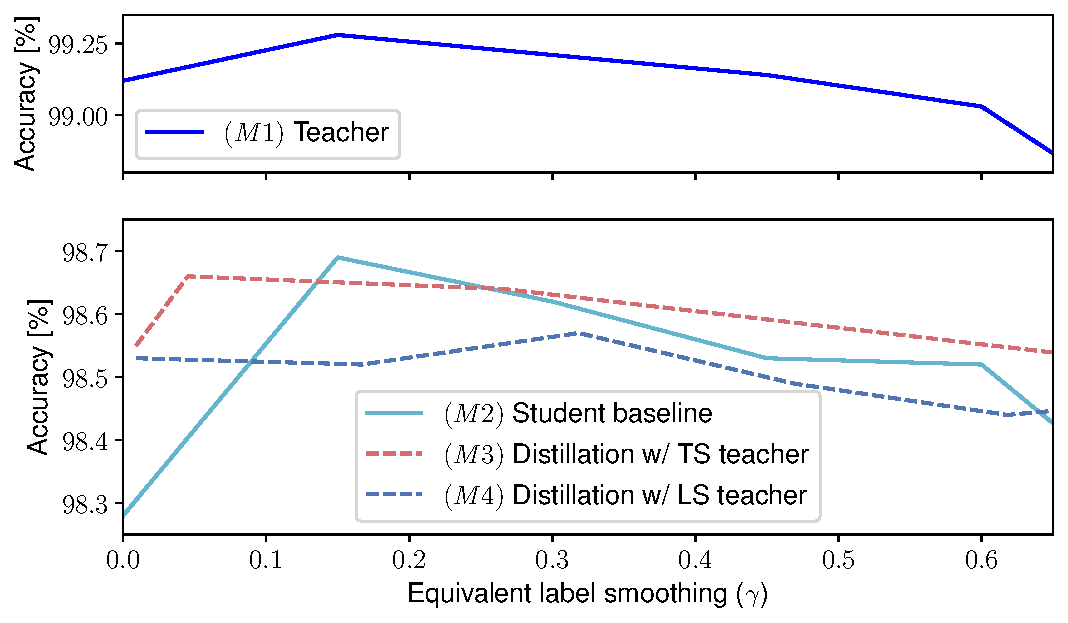
\includegraphics[width=0.8\textwidth]{figures/fc_knowledge_distillation.pdf}
\caption{Performance of distillation from fully-connected architecture ($1200$ neurons) to fully-connected architecture ($800$ neurons) on MNIST.}
\label{fig:fc_dist}
\end{figure}

The results of this experiment are displayed in Figure \ref{fig:fc_dist}. For $(M1)$ and $(M2)$, $\gamma$ is equivalent to $\alpha$, while Definition (\ref{eq:dist_smooth}) was applied to $(M3)$ and $(M4)$. Here one can see that the accuracy of the student baseline $(M2)$ is generally lower than the accuracy of the distillation with a temperature-scaled teacher $(M3)$. Furthermore, the conclusion that the student's accuracy decreases when the teacher is trained with label smoothing remains true when comparing $(M3)$ and $(M4)$.

\subsection{Distillation with Convolutional Networks}
The authors also conducted the above-mentioned experiment on convolutional networks, using ResNet-56 networks as teachers and AlexNet networks as students. The dataset used was CIFAR-10.

\begin{figure}[ht]
\centering
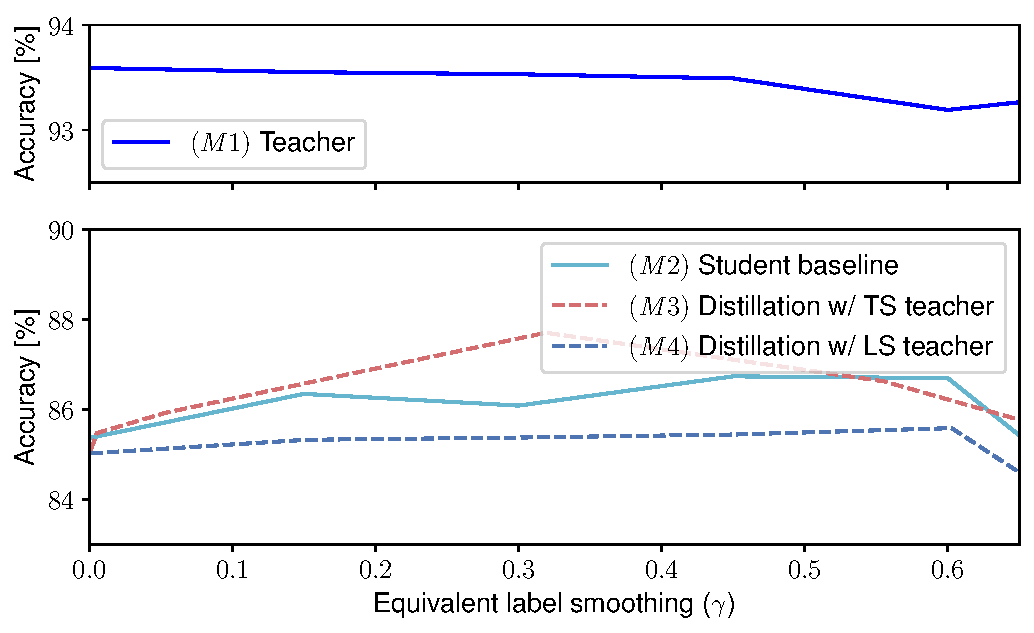
\includegraphics[width=0.8\textwidth]{figures/knowledge_distillation.pdf}
\caption{Performance of distillation from ResNet-56 to AlexNet on CIFAR-10.}
\label{fig:conv_dist}

\end{figure}
Our evaluation results for the models are presented in Figure \ref{fig:conv_dist}. Although the overall results remain consistent, we noticed some discrepancies. While our teachers perform better overall than those in the paper, the accuracy does not improve when using label smoothing. In contrast, the student baseline showed a slight improvement when using label smoothing, which differs from the paper. 
As expected, the use of knowledge distillation with a temperature-scaled teacher enhanced the student's overall accuracy. Furthermore, the accuracy was negatively impacted when the student network was trained via distillation from a teacher using label smoothing. These results confirm the authors' statements and align with the described behavior in the paper.

\subsection{Mutual Information}
To further investigate the reasons for the worse performance when applying label smoothing to a teacher network, the authors compared the amount of information that is erased during the training with label smoothing. This is done by calculating the \textit{mutual information} between the inputs and logits of the network which uses data augmentation as a source of randomness.
Unfortunately, we were unable to reproduce the results from the original work using the described formula. We contacted the authors for clarification but we did not receive an answer.

\section{Conclusion}
In this report, we aimed to reproduce the results of the paper \cite{mueller2019}, which analyzed the impact of label smoothing on classification tasks, while we also provided a deeper insight into label smoothing.
We successfully re-implemented the majority of the experiments from the paper in PyTorch and provided a concrete mathematical description of the penultimate layer visualization which was omitted in the original work.
In detail, by comparing models trained with and without label smoothing, we were able to show that using smooth labels improves the accuracy of the models in most cases.
Furthermore, we demonstrated that the penultimate layer representation of models trained with label smoothing exhibits more compact and better-structured clusters.
We also confirmed the positive impact of label smoothing on model calibration for most classification cases. However, models that were already well-calibrated showed minimal to no improvements when trained on smooth labels. Due to resource constraints, validating the results for ImageNet on InceptionV4 was not feasible.
We applied label smoothing to the training of our transformer model on a smaller dataset than the one used by the original authors.
This resulted in an improvement of the model calibration and did not improve the translation quality.
Furthermore, our findings confirm that using label smoothing in knowledge distillation has a negative impact on the accuracy of the student network. To support this claim, we expanded the experiment using additional models and datasets.
In conclusion, we were able to reproduce a majority of the findings of Müller et al. \cite{mueller2019} and validate the described behavior of label smoothing. In the cases of mutual information and experiments on the Transformer, we were not able to reproduce the results. 